% !TEX encoding = UTF-8 Unicode
% -*- coding: UTF-8; -*-
% vim: set fenc=utf-8
\documentclass[a4paper,12pt,fleqn]{article}
\usepackage[a4paper, total={6.5in, 9in}]{geometry}

\usepackage{multirow}
\usepackage[table,xcdraw]{xcolor}
\usepackage{centrale}
\usepackage{minted}
\usepackage{enumitem}
\usepackage[thinlines]{easytable}
\usepackage{graphicx}       % provides commands for including figures
\usepackage{csquotes}       % provides \enquote{} macro for "quotes"
\usepackage{glossaries}     % provides glossary commands

\usetikzlibrary{matrix,backgrounds}

\newcommand\ezskip{\medskip\noindent}

\lstset{
    frame=tb, % draw a frame at the top and bottom of the code block
    tabsize=4, % tab space width
    showstringspaces=false, % don't mark spaces in strings
    numbers=left, % display line numbers on the left
    commentstyle=\color{green}, % comment color
    keywordstyle=\color{blue}, % keyword color
    stringstyle=\color{red} % string color
}

\hypersetup{
    pdftitle={APP2 Report},
    pdfauthor={Habib Slim, Sofiane Tanji, Eslam Mohammed, Archit Yadav, Albert Strümpler, Manuel Treutlein},
    pdfsubject={Problem Solving},
    pdfproducer={},
    pdfkeywords={greedy, dynamic programming, complete solution space exploration, holdem, cards} %
}

\DeclareGraphicsRule{.ai}{pdf}{.ai}{} % pour insérer des documents .ai
\graphicspath{ {./img/} {./eps/}} % pour ne pas avoir à ajouter eps/ton-image.jpg

% ------------- Packages spéciaux, nécessaires pour ce rapport, à insérer ici ------------- 

\makeglossaries
\newglossaryentry{deque} {
	name = double ended linked list,
	description = {Standard data structure in algorithms. Each element in the list
								 is linked by a pointer to the left and a pointer to the right element, exept
								 the first and the last element. We can access the list only through a pointer
								 on the first and last element.}
}
\newglossaryentry{pop} {
	name = pop(),
	description = {Get the last element in the deque. In terms of the card game this
								 is the rightmost card.}
}
\newglossaryentry{popleft} {
	name = popleft(),
	description = {Get the first element in the deque. In terms of the card game this
								 is the leftmost card.}
}
\newglossaryentry{greedy} {
	name = greedy algorithm,
	description = {The greedy algorithm is a heuristic algorithm pattern to solve
								 problems through making optimal local choices. This might not
								 be optimal in the global context.}
}

\begin{document}

% --------------------------------------------------------------
%                       Page de garde
% --------------------------------------------------------------

\begin{titlepage}
\begin{center}


\includegraphics[width=0.35\textwidth]{logo-uga.png}
\includegraphics[width=0.35\textwidth]{logoinp.png} \\[1cm]

{\large Master M1 MOSIG – UGA \& Grenoble INP} \\[0.8cm]
{\large Algorithmic Problem Solving}\\[0.5cm]

% Title
\rule{\linewidth}{0.5mm} \\[0.4cm]
{ \huge \bfseries APP2: Hold’em for n00bs \\[0.4cm] }
\rule{\linewidth}{0.5mm} \\[1.5cm]

% Author and supervisor
\noindent
\begin{minipage}{0.4\textwidth}
  \begin{flushleft} \large
    \emph{Authors :}\\
    Habib \textsc{Slim}\\
    Eslam \textsc{Mohammed}\\
    Archit \textsc{Yadav}\\
    Albert \textsc{Strümpler}\\
    Manuel \textsc{Treutlein}\\
    Sofiane \textsc{Tanji}
  \end{flushleft}
\end{minipage}%
\begin{minipage}{0.4\textwidth}
  \begin{flushright} \large
    \emph{Teacher :} \\
    Ms.~Malin \textsc{Rau}\\
  \end{flushright}
\end{minipage}

\vfill

% Bottom of the page
{\large Last Version \\ \today}

\end{center}
\end{titlepage}

% --------------------------------------------------------------
%                    Table des matières 
% --------------------------------------------------------------

\thispagestyle{empty}
\tableofcontents
\newpage
% --------------------------------------------------------------
%                         Début du corps
% --------------------------------------------------------------
\section{Introduction}
% Explanation of the problem and modelling.
In this APP we have to deal with a card game played by two persons.
One player is referred to as sister, the other player is referred to as strategist.

THIS PART MUST BE MODIFIED !
--------------------------------------------------
A series of n cards lying on the table face up in a line. We are modelling
the card deck through a \gls{deque}, short deque. The elements of the deque are integers
in the range of [2, 14], whereas the value 2 represents the card 2 and the
value 14 represents the value of an ace. All values in between are assigned
appropriately, this means in particular for the face cards that the jack
is modeled by 11, the queen by 12 and the king by 13.

The deque allows according to the game rules to take only the
rightmost or the leftmost card. The players take turns while playing the
game and always decide to take the leftmost or rightmost card. This is
modeled through \gls{popleft} to take leftmost card and through \gls{pop}
to take the rightmost card. Be careful, the naming of \gls{pop} for taking
the rightmost card can be considered not consistent with \gls{popleft}, but we
stick to the denotation of the phyton standard library. The player with
the highest score in the end wins. Even though we will apply different
algorithms to solve the problem, the input and ouput of the algorithm stays the same.
%% TODO change this section if input or ouput should be different
The input is a list of cards represented as deque and the choice (of the sister)
who starts the game represented as boolean. The output is 0 if the sister wins
or the sum of the players are equal. The output is 1 if the
player strategist wins.\\
--------------------------------------------------

--------> Is this necessary ?
In this APP we decided to change to python code for representing algorithms.
The reason for this is that python code has a simple structure and resembles
pseudo-code in a way. But furthermore it allows us to represent the developed
algorithms more detailed.\\
--------------------------------------------------

The sister will always play the so called \gls{greedy}. Therefore we first consider an algorithm applying this method in chapter 2. Because of some limitations of the \gls{greedy} we will then consider a complete solution space exploration in chapter 3. This gives us an optimal solution, but with an unacceptable runtime. For this reason we will introduce a dynamic algorithm in chapter 4, resulting in an optimal solution with acceptable runtime.

\newpage
\section{Notations}

For all of what follows, we will be using the same data structure to represent the playing cards : a simple array of fixed size containing all card costs that have been drawn, unordered, named "\texttt{CARDS}".

In order to visually describe a configuration of cards in a game, we will be using the following diagram notations :

\begin{figure}[H]
    \centering
    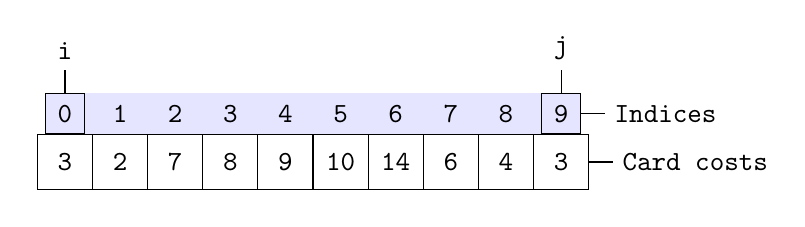
\begin{tikzpicture}[font=\ttfamily,
    array/.style={matrix of nodes,nodes={draw, minimum size=7mm},column sep=-\pgflinewidth, row sep=0mm, nodes in empty cells,
    row 1/.style={nodes={draw=none, fill=none, minimum size=5mm}},
    row 1 column 1/.style={nodes={draw}},
    row 1 column 10/.style={nodes={draw}}}]
    
    \matrix[array] (array) {
    0 & 1 & 2 & 3 & 4 & 5 & 6 & 7 & 8 & 9\\
    3 & 2 & 7 & 8 & 9 & 10&14 & 6 & 4 & 3\\};
    
    \begin{scope}[on background layer]
    \fill[blue!10] (array-1-1.north west) rectangle (array-1-10.south east);
    \end{scope}
    
    \draw (array-1-1.north)--++(90:3mm) node [above] (first) {\textbf{i}};
    \draw (array-1-10.north)--++(90:3mm) node [above] (first) {\textbf{j}};
    \draw (array-1-10.east)--++(0:3mm) node [right]{Indices};
    \draw (array-2-10.east)--++(0:3mm) node [right]{Card costs};
    %
    \end{tikzpicture}
    \caption{Initial configuration}
    \label{fig:example_diag_01}
\end{figure}

More generally, a configuration $(i,j)$ describing a situation produced from a set of $n$ cards is such that :

$$ (i,j) \in [\![0,\ n-1]\!]^2, \ i \leq j $$

If $i$ is equal to $j$, we are describing a configuration in which a single card of index $i$ and of cost \texttt{CARDS[j]} is remaining.

\medskip

Referring to the subconfiguration $(i+1,\ j)$ thus describes a subsequent configuration in which the first player picked the left-most card (here, of cost 3), like shown in figure \ref{fig:example_diag_02}.

\begin{figure}[H]
    \centering
    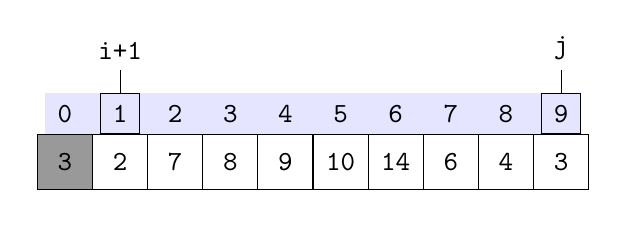
\begin{tikzpicture}[font=\ttfamily,
    array/.style={matrix of nodes,nodes={draw, minimum size=7mm},column sep=-\pgflinewidth, row sep=0mm, nodes in empty cells,
    row 1/.style={nodes={draw=none, fill=none, minimum size=5mm}},
    row 1 column 2/.style={nodes={draw}},
    row 1 column 10/.style={nodes={draw}}}]
    
    \matrix[array] (array) {
    0 & 1 & 2 & 3 & 4 & 5 & 6 & 7 & 8 & 9\\
    3 & 2 & 7 & 8 & 9 & 10&14 & 6 & 4 & 3\\};
    
    \begin{scope}[on background layer]
    \fill[blue!10] (array-1-1.north west) rectangle (array-1-10.south east);
    \fill[gray!80] (array-2-1.north west) rectangle (array-2-1.south east);
    \end{scope}
    
    \draw (array-1-2.north)--++(90:3mm) node [above] (first) {\textbf{i+1}};
    \draw (array-1-10.north)--++(90:3mm) node [above] (first) {\textbf{j}};
    %
    \end{tikzpicture}
    \caption{Following subconfiguration}
    \label{fig:example_diag_02}
\end{figure}

The card of index 0 and of cost 3 has been greyed out, which means that it was selected and can no longer be picked and added to a player's score.

\medskip

In general, referring to the subconfiguration $(i+n,\ j-k)$ describes a configuration in which $n$ cards have been picked on the left-side of the stack, and $k$ cards have been picked on the right side. The constraint $i+n \leq j-k$ must obviously still be correct for the configuration to be valid.

% --------------------------------------------------------------
%                         Partie 1
% --------------------------------------------------------------

\newpage

\section{The greedy algorithm}
%% TODO complete, RESPONSIBLE PERSON: Albert
-- Section 2 basically

\subsection{Pseudocode}
%% TODO complete, RESPONSIBLE PERSON: Sofiane
-- write down the python pseudocode

\subsection{Complexity}
%% TODO complete, RESPONSIBLE PERSON: Sofiane
-- short chapter about the complexity, maybe not necessary.

\subsection{Limitations and advantages}
%% TODO complete, RESPONSIBLE PERSON: Manuel
-- maybe make a table


% --------------------------------------------------------------
%                         Partie 2
% --------------------------------------------------------------

\newpage

\section{Complete solution space exploration}
%% TODO complete, RESPONSIBLE PERSON: Albert
To find a complete solution space exploration

\subsection{Pseudocode}
%% TODO complete, RESPONSIBLE PERSON: Habib, Jimmy
-- write down the python pseudocode

\subsection{Complexity}
%% TODO complete, RESPONSIBLE PERSON: Achret
-- short chapter about the complexity.

%% \subsection{Discussion about possible filters.}
%% TODO ONLY if we have time.
%% TODO complete, RESPONSIBLE PERSON:
%% -- short chapter about the complexity.


% --------------------------------------------------------------
%                         Partie 2
% --------------------------------------------------------------

\newpage


\section{Dynamic Programming solution} \label{sec:dp_solution}
%% TODO complete, RESPONSIBLE PERSON: Jimmy, Habib
The dynamic programing technique is used primarily for optimization problems, where we wish to find the best way of doing something which often the way of doing that something is exponential.
-- "which often the way of doing that something is exponential" => weird sentence maybe ?

Our problem solving process should involve three components:
%% STYLE: put these points in itemized bold way
\begin{itemize}
    \item \textbf{Simple Subproblems}: We must find a way of breaking the global problem into subproblems, each having the same structure to the global problem.
    \item \textbf{Subproblem Optimality}: In order to find the global optimum solution, an optimal solution for each subproblem should be composed.
    \item \textbf{Subproblem Overlapping}: Optimal solutions to unrelated subproblems can contain subproblems in common. Indeed, such overlap allows us to improve the efficiency of a dynamic programming algorithm by storing solutions to subproblems. This last property is particularly important for dynamic programming algorithms, because it allows them to take advantage of memoization, which is an optimization that allows us to avoid repeated recursive calls by storing intermediate values.
\end{itemize}

%% BONUS: add the proof for DP here

To make the problem easier, we make some assumptions about the behavior of players in some undefined situations :

\begin{itemize}
    \item If the sister player has to choose between two cards of equal cost, she always picks the right-most card
    \item If the strategist player has to choose between two cards that yield equal potential scores, he picks the right-most card as well \footnote{\ As shown later on, this assumption has no impact on accurately predicting win or loss.}
\end{itemize}

In the last part \ref{sub:extensions} we attempt to produce a more general version of our dynamic programming approach, getting rid of unnecessary assumptions.

\subsection{First recursive solution}

To begin to solve the problem, we suggest a first solution that does not make use of dynamic programming techniques such as memoization and tabulation. It is a recursive method that finds the optimal solution for the strategist player, under the assumptions mentioned in the introduction of section \ref{sec:dp_solution}.

\subsubsection{Subproblem decomposition} \label{sub:subproblems}
\ezskip
We will consider for each configuration two variables \texttt{firstScore} and \texttt{secondScore} which are equal to the \textbf{final} score\footnote{\ That is, the score obtained after the whole game has been played from this configuration.} of the player making respectively the first, and the second move from this configuration.
To introduce this solution, let us consider the simple configuration described in figure \ref{fig:recursive_01}.

\begin{figure}[H]
    \centering
    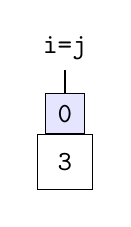
\begin{tikzpicture}[font=\ttfamily,
    array/.style={matrix of nodes,nodes={draw, minimum size=7mm},column sep=-\pgflinewidth, row sep=0mm, nodes in empty cells,
    row 1/.style={nodes={draw=none, fill=none, minimum size=5mm}},
    row 1 column 1/.style={nodes={draw}}}]
    
    \matrix[array] (array) {
    0 \\
    3 \\};
    
    \begin{scope}[on background layer]
    \fill[blue!10] (array-1-1.north west) rectangle (array-1-1.south east);
    \end{scope}
    
    \draw (array-1-1.north)--++(90:3mm) node [above] (first) {\textbf{i=j}};
    %
    \end{tikzpicture}
    \caption{Configuration $(0,0)$}
    \label{fig:recursive_01}
\end{figure}

Let $rem_0$, $rem_1$ be the remaining points that the first player, second player (respectively) are yet to earn in the subsequent configurations.
After this configuration is played (no matter which of the sister or the strategist is playing), the resulting scores will be \texttt{firstScore = 3 + $rem_0$} and \texttt{secondScore = 0 + $rem_1$}.

However, since all cards have been picked, we have $rem_0 = rem_1 = 0$ and the game ends. This simple observation can be extended in a configuration with two playing cards, like shown in figure \ref{fig:recursive_02} :

\begin{figure}[H]
    \centering
    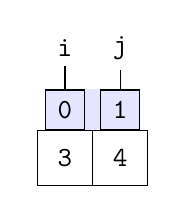
\begin{tikzpicture}[font=\ttfamily,
    array/.style={matrix of nodes,nodes={draw, minimum size=7mm},column sep=-\pgflinewidth, row sep=0mm, nodes in empty cells,
    row 1/.style={nodes={draw=none, fill=none, minimum size=5mm}}
    , row 1 column 1/.style={nodes={draw}}
    , row 1 column 2/.style={nodes={draw}}
    }]
    
    \matrix[array] (array) {
    0 & 1\\
    3 & 4\\};
    
    \begin{scope}[on background layer]
    \fill[blue!10] (array-1-1.north west) rectangle (array-1-2.south east);
    \end{scope}

    \draw (array-1-1.north)--++(90:3mm) node [above] (first) {\textbf{i}};
    \draw (array-1-2.north)--++(90:2.5mm) node [above] (first) {\textbf{j}};
    %
    \end{tikzpicture}
    \caption{Configuration $(0,1)$}
    \label{fig:recursive_02}
\end{figure}

Again, the resulting scores after this configuration will be \texttt{firstScore = 4}\ and \texttt{secondScore = 3}, no matter who the first player is.
We have \texttt{firstScore = 3 + rem\_0} and \texttt{secondScore = rem\_1}. Here however, the subsequent configuration is not empty, and is the configuration $(0,0)$ described in \ref{fig:recursive_01}.
The second player in configuration $(0,1)$ becomes the first player in subconfiguration $(0,0)$, and we then have :

$$firstScore_{(0,1)} = CARDS[1] + rem_0 = CARDS[1] + secondScore{(0,0)} = 4 + 0 = 4$$
$$secondScore_{(0,1)} = rem_1 = firstScore{(0,0)} = CARDS[0] = 3$$

\newpage
Now, if we extend again our configuration with two more cards, we get :

\begin{figure}[H]
    \centering
    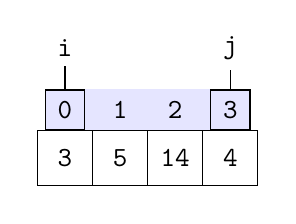
\begin{tikzpicture}[font=\ttfamily,
    array/.style={matrix of nodes,nodes={draw, minimum size=7mm},column sep=-\pgflinewidth, row sep=0mm, nodes in empty cells,
    row 1/.style={nodes={draw=none, fill=none, minimum size=5mm}}
    , row 1 column 1/.style={nodes={draw}}
    , row 1 column 4/.style={nodes={draw}}
    }]
    
    \matrix[array] (array) {
    0 & 1 & 2  & 3\\
    3 & 5 & 14 & 4\\};
    
    \begin{scope}[on background layer]
    \fill[blue!10] (array-1-1.north west) rectangle (array-1-4.south east);
    \end{scope}

    \draw (array-1-1.north)--++(90:3mm) node [above] (first) {\textbf{i}};
    \draw (array-1-4.north)--++(90:2.5mm) node [above] (first) {\textbf{j}};
    %
    \end{tikzpicture}
    \caption{Configuration $(0,3)$}
    \label{fig:recursive_03}
\end{figure}

Let's assume that the first player picks the left-most card. His score for configuration $(0,3)$ will be equal to :

$$firstScore_{(0,3)} = CARDS[0] + rem_0 = 3 + rem_0 $$

The second player's score will then simply be :

$$secondScore_{(0,3)} = rem_1$$

Since he didn't get to pick any card for this configuration.

However, for the next configuration we have :

\begin{figure}[H]
    \centering
    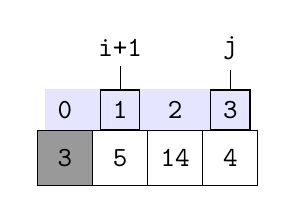
\begin{tikzpicture}[font=\ttfamily,
    array/.style={matrix of nodes,nodes={draw, minimum size=7mm},column sep=-\pgflinewidth, row sep=0mm, nodes in empty cells,
    row 1/.style={nodes={draw=none, fill=none, minimum size=5mm}}
    , row 1 column 2/.style={nodes={draw}}
    , row 1 column 4/.style={nodes={draw}}
    }]
    
    \matrix[array] (array) {
    0 & 1 & 2  & 3\\
    3 & 5 & 14 & 4\\};
    
    \begin{scope}[on background layer]
    \fill[blue!10] (array-1-1.north west) rectangle (array-1-4.south east);
    \fill[gray!80] (array-2-1.north west) rectangle (array-2-1.south east);
    \end{scope}

    \draw (array-1-2.north)--++(90:3mm) node [above] (first) {\textbf{i+1}};
    \draw (array-1-4.north)--++(90:2.5mm) node [above] (first) {\textbf{j}};
    %
    \end{tikzpicture}
    \caption{Configuration $(1,3)$}
    \label{fig:recursive_04}
\end{figure}

\noindent
Let \texttt{$firstScore_{(1,3)}$}, \ \texttt{$secondScore_{(1,3)}$} be the scores for the players in this configuration $(1,3)$. Again, we notice that the first player to pick a card for this configuration was the second player to pick a card in previous configuration $(0,3)$ (figure \ref{fig:recursive_04}), and vice versa. This means that we have :

    \begin{equation}
    \begin{cases}

    firstScore_{(0,3)} = CARDS[0] + rem_0 = CARDS[0] + secondScore_{(1,3)} \\
    secondScore_{(0,3)} = rem_1 = firstScore_{(1,3)}
    
    \end{cases}
    \end{equation}

\ezskip
More generally, with $(i,j)$ being the initial configuration, $(n,k)$ being the immediately subsequent configuration and $\alpha \in \{i,j\}$ being the choice of the first player in configuration $(i,j)$, we have if $i \neq j$:

    \begin{equation}
    firstScore_{(i,j)} =    \begin{cases}
                                CARDS[i] + secondScore_{(i+1,j)}, & \text{if}\ \alpha=i \\
                                CARDS[j] + secondScore_{(i,j-1)}, & \text{else if}\ \alpha=j
                            \end{cases}
    \end{equation}
    \begin{equation} \label{eq:secondScore}
    secondScore_{(i,j)} =    \begin{cases}
                                firstScore_{(i+1,j)}, & \text{if}\ \alpha=i \\
                                firstScore_{(i,j-1)}, & \text{else if}\ \alpha=j
                            \end{cases}
    \end{equation}
    
If $i = j$, as described in figure \ref{fig:recursive_01}, we have :

    \begin{equation}
    firstScore_{(i,j)} = CARDS[i]
    \\
    secondScore_{(i,j)} = 0
    \end{equation}

\subsubsection{Recursive formula} \label{susub:recursive_formula}

Using the definitions and observations made in section \ref{sub:subproblems}, we can start writing the recursive formulas defining the resulting scores of configurations for both players, dealing with the two possible cases :

\begin{itemize}
    \item The first player for configuration $(i,j)$ is the sister
    \item The first player for configuration $(i,j)$ is the strategist
\end{itemize}

If the first player for configuration $(i,j)$ is the sister, she always takes the card between $i$ and $j$ that yields the highest value.
Following our assumptions, if the two cards are of equal cost, she picks the right-most card.

We then have for the \texttt{firstScore}\footnote{\ \texttt{secondScore} is still defined as in equation \ref{eq:secondScore} with $\alpha$ being equal to i in first case, and j in the second} :

    \begin{equation}
    firstScore_{(i,j)} =    \begin{cases}
                                CARDS[i] + secondScore_{(i+1,j)} & \text{if CARDS[i] > CARDS[j]} \\
                                CARDS[j] + secondScore_{(i,j-1)} & \text{otherwise}
                            \end{cases}
    \end{equation}
    
If the first player is the strategist however, he must pick the card that yields a greater global score.
This global score can be written as such :

    \begin{equation}
    firstScore_{(i,j)} = \max \left(CARDS[i] + secondScore_{(i+1,j)}, \ 
                                    CARDS[j] + secondScore_{(i,j-1)}\right)
    \end{equation}

\subsubsection{Recursive implementation}

Our implementation for this version of the program is very straightforward and comes directly from our recursion formula. We first define the global constants of our program.

\begin{itemize}
    \item \texttt{CARDS} is an array containing all cards as described in the introduction
    \item \texttt{LEN\_CARDS} is the total number of cards (equal to $n$)
    \item \texttt{SISTER\_FIRST} is a boolean, which is equal to true if the sister picks a card first
\end{itemize}

\ezskip Let $getScores$ be a function operating on configurations of list \texttt{CARDS} that takes as parameters :

\begin{itemize}
    \item \texttt{i,j} : The configuration indexes
    \item \texttt{sister\_first} : equals to true if the sister is the one to pick a card for this configuration
\end{itemize}

And returns a tuple :

$$getScore(i, j, sisterFirst) = (firstScore,\ secondScore)$$

\noindent \texttt{(firstScore, secondScore)} being the total score of the first and second players for the configuration $(i,j)$ if the sister start first or not, \textbf{in the optimal case for the strategist}.
This means that if \texttt{sisterFirst = true}, \texttt{firstScore} is the sister's score and vice-versa.
Thus \texttt{firstScore} > \texttt{secondScore} means that the sister won for configuration $(i,j)$.

We then implement the recursive formulas defined in section \ref{susub:recursive_formula} :

\begin{minted}[frame=leftline]{Python}
def getScores(i, j, sisterFirst):
    if (i==j): return (CARDS[i], 0)
    if (sisterFirst):
        # Sister takes the card of superior cost (local optimum)
        if (CARDS[i] > CARDS[j]):
            scoreTuple = getScores(i+1, j, not sisterFirst)
            firstScore  = CARDS[i] + scoreTuple[1]
            secondScore = scoreTuple[0]
        else:
            scoreTuple = getScores(i, j-1, not sisterFirst)
            firstScore  = CARDS[j] + scoreTuple[1]
            secondScore = scoreTuple[0]
    else:
        leftCardScore = getScores(i+1, j, not sisterFirst)
        rightCardScore = getScores(i, j-1, not sisterFirst)

        # Strategist takes the card that leads to better score (global optimum)
        if (CARDS[i] + leftCardScore[1] > CARDS[j] + rightCardScore[1]):
            firstScore = CARDS[i] + leftCardScore[1]
            secondScore = leftCardScore[0]
        else:
            firstScore = CARDS[j] + rightCardScore[1]
            secondScore = rightCardScore[0]
    
    return (firstScore, secondScore)
\end{minted}

As an example, we will re-use the following configuration :

\begin{figure}[H]
    \centering
    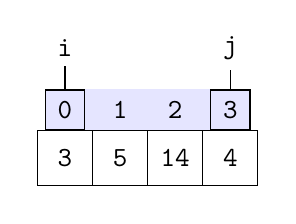
\begin{tikzpicture}[font=\ttfamily,
    array/.style={matrix of nodes,nodes={draw, minimum size=7mm},column sep=-\pgflinewidth, row sep=0mm, nodes in empty cells,
    row 1/.style={nodes={draw=none, fill=none, minimum size=5mm}}
    , row 1 column 1/.style={nodes={draw}}
    , row 1 column 4/.style={nodes={draw}}
    }]
    
    \matrix[array] (array) {
    0 & 1 & 2  & 3\\
    3 & 5 & 14 & 4\\};
    
    \begin{scope}[on background layer]
    \fill[blue!10] (array-1-1.north west) rectangle (array-1-4.south east);
    \end{scope}

    \draw (array-1-1.north)--++(90:3mm) node [above] (first) {\textbf{i}};
    \draw (array-1-4.north)--++(90:2.5mm) node [above] (first) {\textbf{j}};
    %
    \end{tikzpicture}
    \caption{Configuration $(0,3)$}
    \label{fig:recursive_05}
\end{figure}

On this configuration, whoever gets the card of cost 14 wins.
If the first player is the sister she will always pick the 4 card, thus giving the strategist immediate win. If the strategist starts, he should pick 3 so that the sister is forced to pick either 5 or 4, thus giving him the win.

\ezskip
Thus, if the sister plays first, the strategist should always win with a score of 14 + 3 = 17, and if the strategist plays first he should win with the same score (picking 3, sister picks 5, strategist picks 14 and wins).

\ezskip
Running this function on this starting configuration with two values for \texttt{sisterFirst} gives us the scores in comments in the following snippet of code :

\begin{minted}[frame=leftline]{Python}
scores = getScores(0, LEN_CARDS - 1, False) # => expected : (17, 9)
scores = getScores(0, LEN_CARDS - 1, True)  # => expected : (9, 17)
\end{minted}

Which are indeed the predicted results for this example (the strategist always wins with a score of 17).

\subsubsection{Complexity}
%% TODO : Write complexity analysis for the first recursive version with a nice diagram : ??

-- EASY - Can be directly taken from the course material

\newpage
\subsection{Memoization and Tabulation}
%% TODO complete, RESPONSIBLE PERSON: Jimmy, Habib
-- WRITE A NICE INTRO (memoization is "optimized recursive version" and tabulation is "sequential version"

\subsubsection{Memoization} \label{susub:memoization}

In order to improve the complexity of our first recursive version, we remove redundant calculations by caching the results of the sub-problems. To achieve this, we allocate a two-dimensional cache of size $n \times n$ that will contain the computed subconfigurations.

In practice, $cache[i][j]$ will yield the tuple \texttt{(firstScore, secondScore)} of configuration $(i,j)$.

\ezskip
Below is the memoized version of our \texttt{getScores} function :

\begin{minted}[frame=leftline]{Python}
cache = [[0]*LEN_CARDS for _ in range(LEN_CARDS)]
def getScores(i, j, sisterFirst):
    if (cache[i][j] != 0): return cache[i][j]
    if (i==j): return (CARDS[i], 0)

    if (sisterFirst):
        # Sister takes the local optimum
        if (CARDS[i] > CARDS[j]):
            scoreTuple = getScores(i+1, j, not sisterFirst)
            firstScore  = CARDS[i] + scoreTuple[1]
            secondScore = scoreTuple[0]
        else:
            scoreTuple = getScores(i, j-1, not sisterFirst)
            firstScore  = CARDS[j] + scoreTuple[1]
            secondScore = scoreTuple[0]
    else:
        leftCutScore = getScores(i+1, j, not sisterFirst)
        rightCutScore = getScores(i, j-1, not sisterFirst)

        # Strategist takes the global optimum
        if (CARDS[i] + leftCutScore[1] > CARDS[j] + rightCutScore[1]):
            firstScore = CARDS[i] + leftCutScore[1]
            secondScore = leftCutScore[0]
        else:
            firstScore = CARDS[j] + rightCutScore[1]
            secondScore = rightCutScore[0]
    
    cache[i][j] = (firstScore, secondScore)
    return cache[i][j]
\end{minted}

Some precisions :
\begin{itemize}
    \item The default value we use for our cache is 0, because an initialized cache entry must contain a tuple object.
    \item Since configurations $(i,j)$ with $i > j$ are impossible, half of our table below the diagonal is unused (as seen in figure \ref{fig:memoization_01}).
    \item Because the sister makes choices only based on the two available cards, and not on the overall score of subconfigurations, some configurations will never be explored.
\end{itemize}

The last point is explained a bit more completely below. In our Python function, we have the following condition :

\begin{minted}[frame=leftline]{Python}
# Sister takes the local optimum
if (CARDS[i] > CARDS[j]): # alpha = i
    scoreTuple = getScores(i+1, j, not sisterFirst)
    firstScore  = CARDS[i] + scoreTuple[1]
    secondScore = scoreTuple[0]
else:                     # alpha = j
    scoreTuple = getScores(i, j-1, not sisterFirst)
    firstScore  = CARDS[j] + scoreTuple[1]
    secondScore = scoreTuple[0]
\end{minted}

If case $\alpha = i$ is taken, then \texttt{getScores(i,j-1)} will never be computed and the subconfiguration $(i, j-1)$ will never be considered\footnote{\ Please refer to figure \ref{fig:tabulation_01} for the dependency graph further justifying this argument.}.

As an illustration, in table \ref{tab:memoization_02} below is an example of the resulting cache of the execution of our optimized recursive function, on the initial configuration described in figure \ref{fig:memoization_01} :

\begin{figure}[H]
    \centering
    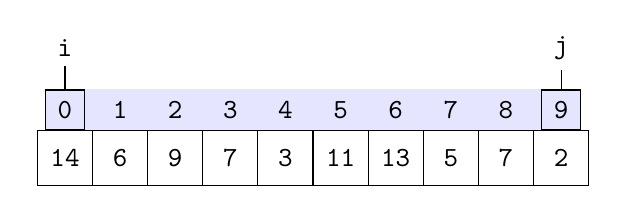
\begin{tikzpicture}[font=\ttfamily,
    array/.style={matrix of nodes,nodes={draw, minimum size=7mm},column sep=-\pgflinewidth, row sep=0mm, nodes in empty cells,
    row 1/.style={nodes={draw=none, fill=none, minimum size=5mm}}
    , row 1 column 1/.style={nodes={draw}}
    , row 1 column 10/.style={nodes={draw}}
    }]
    
    \matrix[array] (array) {
    0 & 1 & 2 & 3 & 4 & 5 & 6 & 7 & 8 & 9\\
    14& 6 & 9 & 7 & 3 & 11& 13& 5 & 7 & 2\\};

    \begin{scope}[on background layer]
    \fill[blue!10] (array-1-1.north west) rectangle (array-1-10.south east);
    \end{scope}

    \draw (array-1-1.north)--++(90:3mm) node [above] (first) {\textbf{i}};
    \draw (array-1-10.north)--++(90:2.5mm) node [above] (first) {\textbf{j}};
    %
    \end{tikzpicture}
    \caption{Configuration $(0,9)$}
    \label{fig:memoization_01}
\end{figure}

\begin{table}[H]
\centering
\begin{TAB}(e,1cm,1cm){|c:c:c:c:c:c:c:c:c:c|}{|c:c:c:c:c:c:c:c:c:c|}
\hline
0         &0         &0         &0         &0         &0         &0         &0         &(43, 32)  &(46, 31) \\
0         &0         &0         &0         &0         &0         &0         &(29, 25)  &(32, 29)  &(31, 32) \\
0         &0         &0         &0         &(12, 7)   &(18, 12)  &(25, 12)  &(25, 23)  &(32, 23)  &(32, 25) \\
0         &0         &0         &(7, 0)    &(7, 3)    &(14, 3)   &0         &(23, 16)  &(23, 23)  &(25, 23) \\
0         &0         &0         &0         &(3, 0)    &(11, 3)   &(16, 3)   &(16, 16)  &(23, 16)  &(23, 18) \\
0         &0         &0         &0         &0         &(11, 0)   &0         &(16, 13)  &0         &(18, 20) \\
0         &0         &0         &0         &0         &0         &(13, 0)   &(13, 5)   &(18, 7)   &(20, 7)  \\
0         &0         &0         &0         &0         &0         &0         &(5, 0)    &(7, 5)    &(7, 7)   \\
0         &0         &0         &0         &0         &0         &0         &0         &(7, 0)    &(7, 2)   \\
0         &0         &0         &0         &0         &0         &0         &0         &0         &(2, 0)   \\
\end{TAB}
\caption{Resulting entries for the memoization cache}
\label{tab:memoization_02}
\end{table}

As expected, on the diagonal we have entries of the form \texttt{(CARDS[i], 0)}. We can also see that entries below the diagonal are never initialized.
Trying to use a data structure that would not leave half of the table uninitialized is not relevant towards space complexity, because it would still be in $O(n^2)$.

\ezskip
As aforementioned, some entries in the memoization cache don't have to be computed because of the sister's greedy strategy.

\subsubsection{Memoization solution complexity}
%% TODO complete, RESPONSIBLE PERSON: Jimmy, Habib

-- EASY : Can be directly taken from the course material

\subsubsection{Tabulation}

Our current complexity is improving, however we would like to optimize our function a bit more by getting rid of recursion overhead.
We start by making a dependency graph of our cache entries. In gray are the entries for the configurations in which the starting player for the global configuration (the upper-right one in the diagram) is the one to pick a card, and in grey are the ones in which the second player becomes the first to make a move.

\begin{figure}[H]
    \centering
    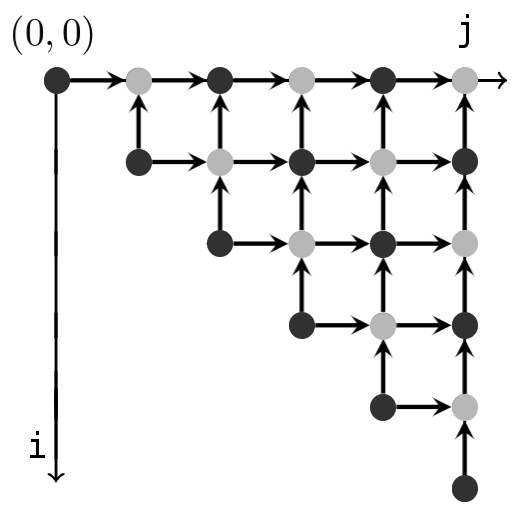
\includegraphics[scale=0.5]{tabulation_01.png}

    \caption{Dependency graph}
    \label{fig:tabulation_01}
\end{figure}

\textbf{Remark :} In a top-down approach, like the one presented in section \ref{susub:memoization}, computing all entries is not mandatory because the sister always picks the local optimum. Some entries of the cache for some subconfigurations will never have to be computed to get an optimal answer, like shown in table \ref{tab:memoization_02}. However, in a bottom-up approach, we will have to compute all entries to get the scores of the final configuration.

\medskip
This does not change the algorithmic complexity which will still be in $O(n^2)$, however it could potentially affect run time. It is a trade-off between getting rid of the recursion overhead and dramatically reducing space complexity (which will be in $O(n)$ for the bottom-up approach), and computing some unnecessary configurations.

\ezskip
To get this bottom-up solution to work, we consider the bottom diagonal and move all the way up to the global configuration.
The first diagonal is initialized easily, with :

\begin{equation}
cache[i][i] = (CARDS[i], 0), \ i \in [\![0,\ n-1]\!] 
\end{equation}

We then move up, computing the next stage using the recurrence formula (as described in \ref{fig:tabulation_02}). To know whether or not each diagonal corresponds to the first or second player (gray and black colors in the diagram), we just compute the modulo of the $j$ index of the current diagonal :

\begin{equation}
(j + n) \equiv_{2} 1 \implies sisterFirst_{diag_j} = sisterFirst_{(0,\ n-1)}
\end{equation}
\begin{equation}
(j + n) \equiv_{2} 0 \implies sisterFirst_{diag_j} = \neg \ sisterFirst_{(0,\ n-1)}
\end{equation}

\begin{figure}[H]
    \centering
    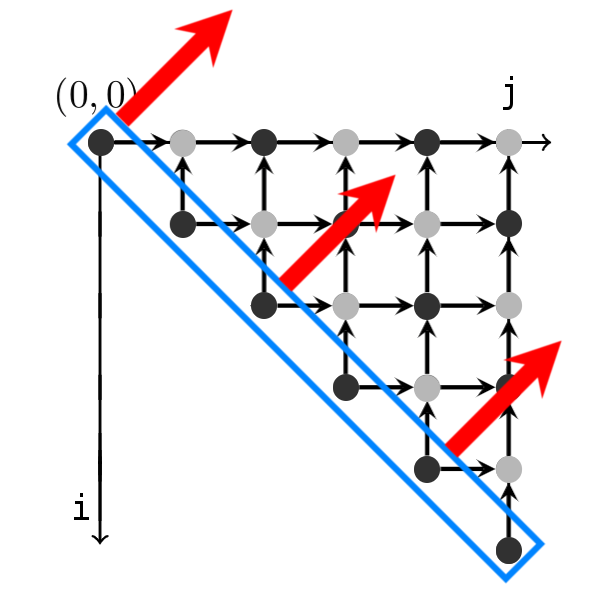
\includegraphics[scale=0.5]{tabulation_02.png}

    \caption{Following the diagonal}
    \label{fig:tabulation_02}
\end{figure}

\noindent
Below is the Python implementation of the bottom-up version of the program :

\begin{minted}[frame=leftline]{Python}
cache = [[0]*LEN_CARDS for _ in range(LEN_CARDS)]
# Finding which player is first on diagonal {diag_index}
def isSisterFirst(diag_index, sisterFirst):
    if ((diag_index + LEN_CARDS)%2 == 1):
        return sisterFirst
    else:
        return not sisterFirst

# Updating a cell value on a diagonal
def updateCell(coord, sisterFirst):
    i,j = coord
    if (sisterFirst):
        # Sister takes the local optimum
        if (CARDS[i] > CARDS[j]):
            firstScore  = CARDS[i] + cache[i+1][j][1]
            secondScore = cache[i+1][j][0]
        else:
            firstScore  = CARDS[j] + cache[i][j-1][1]
            secondScore = cache[i][j-1][0]
    else:
        # Strategist takes the global optimum
        if (CARDS[i] + cache[i+1][j][1] > CARDS[j] + cache[i][j-1][1]):
            firstScore = CARDS[i] + cache[i+1][j][1]
            secondScore = cache[i+1][j][0]
        else:
            firstScore = CARDS[j] + cache[i][j-1][1]
            secondScore = cache[i][j-1][0]
    
    cache[i][j] = (firstScore, secondScore)

def getScores(i, j, sisterFirst):
    if (i==j): return (CARDS[i], 0)

    # Initializing the main diagonal
    for k in range(LEN_CARDS):
        cache[k][k] = (CARDS[k], 0)

    # Computing all cache values diagonal by diagonal
    for diag_index in range(1, LEN_CARDS):
        sisterFirstDiag = isSisterFirst(diag_index, sisterFirst)

        # Updating all cells in the diagonal
        it_coord = [0, diag_index]
        for _ in range(LEN_CARDS - diag_index):
            updateCell(it_coord, sisterFirstDiag)
            it_coord = [x+1 for x in it_coord]

    return cache[0][LEN_CARDS-1]
\end{minted}

No more recursive calls are necessary to obtain the optimal score for the strategist, however we now need to compute every cache value.
As an example, in table \ref{tab:tabulation_03} is the cache obtained when executing this new bottom-up function on the configuration of the aformentioned figure \ref{fig:memoization_01} (as a reminder, table \ref{tab:memoization_02} was the final cache using the top-bottom solution).

\ezskip
This new version of the function returns exactly the same optimal scores and intermediate scores for subconfigurations, however it makes a lot more computations than the top-bottom version. The complexity however still remains the same, and we got rid of the recursion overhead.

\begin{table}[H]
\centering
\begin{TAB}(e,1cm,1cm){|c:c:c:c:c:c:c:c:c:c|}{|c:c:c:c:c:c:c:c:c:c|}
\hline
(14, 0)   &(14, 6)   &(20, 9)   &(23, 13)  &(26, 13)  &(27, 23)  &(37, 26)  &(39, 29)  &(43, 32)  &(46, 31) \\
0         &(6, 0)    &(9, 6)    &(13, 9)   &(13, 12)  &(23, 13)  &(26, 23)  &(29, 25)  &(32, 29)  &(31, 32) \\
0         &0         &(9, 0)    &(9, 7)    &(12, 7)   &(18, 12)  &(25, 18)  &(25, 23)  &(32, 23)  &(32, 25) \\
0         &0         &0         &(7, 0)    &(7, 3)    &(14, 7)   &(20, 14)  &(23, 16)  &(23, 23)  &(25, 23) \\
0         &0         &0         &0         &(3, 0)    &(11, 3)   &(16, 11)  &(16, 16)  &(23, 16)  &(23, 18) \\
0         &0         &0         &0         &0         &(11, 0)   &(13, 11)  &(16, 13)  &(20, 16)  &(18, 20) \\
0         &0         &0         &0         &0         &0         &(13, 0)   &(13, 5)   &(18, 7)   &(20, 7)  \\
0         &0         &0         &0         &0         &0         &0         &(5, 0)    &(7, 5)    &(7, 7)   \\
0         &0         &0         &0         &0         &0         &0         &0         &(7, 0)    &(7, 2)   \\
0         &0         &0         &0         &0         &0         &0         &0         &0         &(2, 0)   \\
\end{TAB}
\caption{Resulting entries for the memoization cache}
\label{tab:tabulation_03}
\end{table}

This solution can be further down optimized in memory to $O(n)$ space complexity by storing only two subsequent diagonals at a time.
Below is the implementation corresponding to this improvement :

-- EASY : Just an easy extension of the previous implementation

\subsubsection{Tabulation solution complexity}

-- EASY : Can be directly taken from the course material

\subsection{Extensions} \label{sub:extensions}
% TODO complete, RESPONSIBLE PERSON: Habib
-- add one version of the algorithm returning the probability of success instead of assuming sister takes choice A or B
-- Maybe I'll look into this later

% --------------------------------------------------------------
%                         Conclusion
% --------------------------------------------------------------

\section{Conclusion and feedback}

%% TODO complete, RESPONSIBLE PERSON: Manuel
-- Write something in general

% --------------------------------------------------------------
%                            Abstract
% --------------------------------------------------------------

\end{document}
